% This is samplepaper.tex, a sample chapter demonstrating the
% LLNCS macro package for Springer Computer Science proceedings;
% Version 2.20 of 2017/10/04
%
\documentclass[runningheads]{llncs}
%
\usepackage{graphicx}
\usepackage[dvipsnames]{xcolor}
% Used for displaying a sample figure. If possible, figure files should
% be included in EPS format.
%
% If you use the hyperref package, please uncomment the following line
% to display URLs in blue roman font according to Springer's eBook style:
% \renewcommand\UrlFont{\color{blue}\rmfamily}

\begin{document}
%
\title{Literary Studies Meet Corpus Linguistics: Estonian Pilot Project of Private Letters in KORP\thanks{Research supported by the institutional research grant ``Formal and Informal Networks of Literature, Based on Sources of Cultural History'' (IRG22-2, Estonian Ministry of Education and Research), related to the Centre of Excellence in Estonian Studies (CEES) and by the programme ASTRA (2014-2020.4.01.16-0026) via the European Regional Development Fund (TK145).  Development of KORP and adding corpora in Estonian is supported by the ERDF project ``Federated Content Search for the Center of Estonian Language Resources'' (2014--2020.4.01.16--0134) under the activity ``Support for Research Infrastructures of National Importance, Roadmap''.}}
%
\titlerunning{Private Letters in KORP}
% If the paper title is too long for the running head, you can set
% an abbreviated paper title here
%
\author{Marin Laak\inst{1} \and Kaarel Veskis\inst{1} \and\\
Olga Gerassimenko\inst{2} \and Neeme Kahusk\inst{2} \and
Kadri Vider\inst{2}}
%
\authorrunning{M. Laak et al.}
% First names are abbreviated in the running head.
% If there are more than two authors, 'et al.' is used.
%
\institute{Estonian Literary Museum\\
  Vanemuise 42, 51003 Tartu, Estonia\\
\email{\{marin.laak,kaarel.veskis\}@kirmus.ee}\and
Institute of Computer Science, University of Tartu,\\
J. Liivi 2, 50409 Tartu, Estonia
\email{\{olga.gerassimenko,neeme.kahusk,kadri.vider\}@ut.ee}
}
%
\maketitle              % typeset the header of the contribution
%
\begin{abstract}
  Digitisation of cultural heritage in Estonia has been in progress during recent years, and we will see expansive mass digitalisation of printed books and handwritten documents in the very near future.
  
  This situation and potential actualises questions of the usage of the literary heritage. In our paper, we consider benefits for digital literary research that arise from representing a literary text collection as an annotated language resource. We discuss the pilot project of creating a text corpus based on private letters between two Estonian avangardist writers in the beginning of the 20th century.
  
The advantages and possibilities of corpus query system KORP that we have chosen for representing and searching literary heritage DH corpora as a language resource are described. Challenges that the application of Natural Language Processing and Text and Data Mining imposes on the preparation and representation of texts are discussed along with benefits for the research. 


\keywords{literary studies \and private letters \and digital heritage collections \and corpus linguistics \and natural language processing}

\end{abstract}
%
%
%
\section{Introduction}

Application of Natural Language Processing (NLP) and Text and Data Mining (TDM) methods and tools is gradually increasing and becoming more relevant in DH research in Estonia. Similarly to the Nordic and Baltic countries, Estonia can expect an explosive growth in digital heritage and text resources: preparations for massive digitisation of cultural heritage started as a national programme in 2019. The creation of these new digital resources will be the priority for all Estonian leading memory institutions and the scope of this huge project includes different types of cultural heritage (printed books, archival documents, photo and film heritage, ethnographic and fine art objects) \cite{digiteerimine,viireslaak18} Digitized resources will be made accessible on the internet as open data, but it is still an open question how and for what purpose can such digital resources be used \cite{laakviires}. 

What are the new challenges and the new knowledge offered by using the tools of NLP in analysing the digital literary heritage? Our interdisciplinary project ``Literary Studies Meet Corpus Linguistics'' concentrates on using cultural heritage, especially literary history sources in research with the help of the NLP\&TDM methods. The primary question is how to bridge the gap between the research possibilities offered by the contemporary NLP\&TDM and the ever increasing amount of digitized texts and other digital data, produced by memory institutions. This has proved to be a complicated task and international practice has shown that literary scholars are slower to embrace new practices than linguists for whom corpus-based research is already a professional standard. In general, literary scholars are used to working with texts using traditional methods, analysing them as undivided poetical and semantic entities \cite{viireslaak18}. Digitizing of texts often preserves them as undivided and unannotated entities with occasionally added metadata - as a result, the digitized materials are human-readable rather than machine-readable.

NLP\&TDM methods require treating literary works or texts as data, which can be analysed and processed with computer programmes. To process data for statistics and for finding trends, a literary scholar needs either to do a close reading of literary texts as huge data amounts, or to develop new professional skills in data analysis methods. This imposes rethinking the approach to empirical object in literary studies in general and posing new and different research questions. The possibility to compare text strategies, rhetorical and stylistic patterns in literary, religious and political text corpora might give us new insights into intertwining ideology, rhetoric and identity presentations. One of the important trends of automated textual analysis in DH is Sentiment Analysis which, for instance, allows to measure emotion in parliamentary debates \cite{Rheault2016}.


\section{Private letters as a literary source}

The empirical foundation of our pilot project of private letters in KORP is based on the archival ego-documents. This is a rare collection of handwritten private letters: the correspondence between two Estonian writers Johannes Semper (1892--1970) and Johannes Barbarus (1890--1946). The authors were well-known avant-garde writers in Estonian literature, best friends and school classmates. They shared the same intellectual attitudes, views, and values. For example, they were Francophiles and during several decades they both reviewed and translated French literature into Estonian. 

During the years covered by the correspondence, in 1911--1939, Barbarus published the total of 17 collections of poetry, and Semper published four collections of poetry and four books of short stories and novels. The letters were written mainly at different locations in Estonia, and also during travels: they both travelled extensively in Europe (and other parts of the world) and in their letters they described to each other the sights they saw as well as the literary events at home. They also wrote about their work, everyday life, health and prescriptions, hobbies (hunting, swimming, skating, etc.), and guests. 

The temporal and contextual frames of this correspondence are the period in Europe between two World Wars and, according to the French philosopher Pierre Bourdieu, the creation of  the Estonian ‘cultural field’ in the Estonian Republic in years 1918--1940. As such, the correspondence offers semantically rich and multidimensional content for literary scholars.  

Generally, we have been inspired by the question how this kind of sources (private letters, correspondences, manuscripts, etc.) in different kinds of machine-readable formats (pdf, docx, txt etc.) can be used for creating new knowledge in the interdisciplinary field of literary studies, including biographics and life writing studies \cite{2015}. 

The private correspondence of two Estonian writers during 28 years, as empirical material, is extremely rich in the themes and possibilities to pose the traditional as well as the new research questions: the factors of subjectivity and emotionality, verbal and poetic creativeness of the both authors, etc.  

The original letters are held at different archives: the letters of Barbarus to Semper belong to the Estonian Cultural History Archives of the Estonian Literary Museum and the letters of Semper to Barbarus belong to the Estonian National Archives due to the unique literary and historical value of this correspondence. Their correspondence consists of 670 letters with, all in all, more than 1,100 pages and more than 310 000 tokens or about 250 000 words.  The number of tokens and words is approximate, as we will discuss later. 


\section{KORP as a tool for corpus linguistics}

KORP is a corpus query analysis system that allows to find concordances and build various statistics from differently annotated corpora using text metadata (author, year of publishing, text type etc) and linguistic annotation (splitting into sentences and words, punctuation, morphology, syntax and semantics). Technically, KORP is a frontend tool that uses much of IMS Open Corpus Workbench \cite{Hardie:2012:1384-6655:380} as backend. It was created and maintained at Swedish Language Bank Spr{\aa}kbanken \cite{BORIN12.248} and is being developed and customised by language technology networks in several countries: Sweden\footnote{ https://spraakbanken.gu.se/korp/}
, Finland\footnote{http://korp.csc.fi}, Norway\footnote{http://gtweb.uit.no/korp/}, Estonia\footnote{http://korp.keeleressursid.ee}, Denmark\footnote{http://alf.hum.ku.dk/korp/} and Island\footnote{http://malheildir.arnastofnun.is/}. 
% Puudu on kõik joonealused urlid nende KORPide kohta!! palun pandagu tagasi! +
% vt Sprakbankeni nullikesega a on valesti vormistatud ja pole print-versioonis näha!! +

Estonian KORP is hosted by the Centre of Estonian Language Resources\footnote{https://www.keeleressursid.ee}. The Estonian data available in KORP currently consists of more than 850 million tokens. As Estonian is a highly inflective language with a rich morphology and free word order, almost all texts are automatically annotated and disambiguated on the morphological level to enable form- and baseform-based search.


As a pilot project for the needs of literary studies in addition to the corpora designed for linguistic research, we have created Correspondence Corpus of private letters (Semper and Barbarus, 1911--1940). The original handwritten manuscripts where already typed in. They were to transform to machine-readable text files by manually adding metadata and automatically analyzing and disambiguating morphological categories. 

KORP as a corpus query system was chosen because of its open source value, search flexibility and easiness, graphical overview of search results in subcorpora, easy switching between concordances and broader context (as well as between frequency statistics and concordances), broad possibilities to group absolute frequencies of tokens or occurrences and automatically calculated relative frequencies (occurrences per million tokens).  Search results and statistics from KORP are exportable into Comma Separated Values (CSV) and JSon format. 
% VÄLJA: we plan to extend the export to the Excel (XLS) and HTML formats (already used in Finnish KORP),  integrate a single sign-on access for corpora with restricted usage, introduce links to audio and video data, links to lexicons and automatic annotation of corpora, the features already implemented in KORP of the other countries (Finland, Sweden, Norway). +

Text fragments cited in KORP are limited to a sentence or a passage, so that KORP does not infringe copyrights. Metadata cited in the query results allow exact pinpointing of the source of the sentence, and it is possible to link whole texts hosted elsewhere to the search metadata for close reading of a broader context when needed. 

KORP helps to analyse and objectively verify or refute different research arguments, for example, such as presented by Estonian literary scholars in the 1980s:
% järgneb loend, palun vormistada!!+ LÕIGU VAHET POLEKS VAJA, mrn
\begin{enumerate}
\item The correspondence of Semper and Barbarus is subjective and emotional, the letters reveal the character and state of mind of the authors at the moment of writing them.

\item The letters demonstrate the authors’ awareness of topical problems in Estonia and in Europe.

\item The subject range of the letters includes everyday life, health, hobbies, visits and visitors, literary work, books and reading, and the literary, economic and political life in Estonia and Europe.
\end{enumerate}

\section{Challenges for annotation in manuscript corpus}

Which distinctive features of older correspondences need to be considered in preparing them to be used as a corpus? Several steps are necessary to convert the digitised text collection into a morphologically analysed corpus, and to provide it with essential metadata about the sources.

\begin{enumerate}
\item The first step in digitising different kinds of manuscripts, incl. private letters, is retyping the handwritten originals in order to transform them into machine-readable format. Digitised typed texts can be subjected to the character recognition (OCR). 

\item In order to enable statistics and to find different linguistic phenomena in the texts, it is important to tokenise at least sentences and words, and to preserve meaningful units (chapters, articles, verses, letters). 

  \item The process of annotation was carried out semi-automatically. At the first stage, sentence boundaries were determined, then words were tokenised. Tokenised words were lemmatised and tagged by part-of-speech and other grammatical features.

\end{enumerate}

Different levels of annotation make it possible to search for different linguistic or other phenomena. In a tokenised text we can search by word forms (or their parts), but not by lemmas. In a lemmatised text we can search also by lemmas, but not by morphological characteristics (e.g., the case, the number). When the text has been morphologically analysed and disambiguated, we can search also by morphological characteristics and parts of speech. The automatic morphological analysis and automatic disambiguation that enable searching for different morphological forms of a word based on the lemma, seriously improve the usability and quality of the corpus. The accuracy of automatic morphological disambiguation in the Estonian standard language corpora reaches up to 93--98\% \cite{veskisliba}.  The accuracy for these texts is propably much lower.


% VÄLJA: The additional clause tokenisation helps to find the linguistic phenomena occurring in the clauses (e.g. the phrasal verbs and idiomatic expressions). The yield and accuracy of automated tokenisation of clauses in the Estonian standard language corpora is, respectively, 95\% and 96\% \cite{Kaalep2012}. 
Meaningful units, e.g., temporal expressions or named entities, found in the text can also be used in searches. If all the meanings of words were tagged, it would be possible to search for a specific meaning of a word and discard all other meanings. 

\section{Annotation types specific for private letters}

The private letters of writers, the correspondence as whole was not addressed for a wider audience. Creators of the corpus met serious difficulties because often, both correspondents were very familiar with the subjects mentioned in the letters, so that sometimes they only hinted at the events or persons and used plenty of abbreviations known only to themselves. Authors of letters reflect both the historical period and the personal context and idiolects. Being avant-garde poets, Semper \& Barbarus both experimented with the language a lot. 
% TÕLKIDA:
% Järgnevalt anname ülevaate iseloomulikest joontest, mis väärivad eraldi annoteerimist uuritavas materjalis. Kõiki annotatsioonitüüpe koos on illustreerivalt kujutatud Fig. 1 +

In the following sections we are going to present the distinctive features of the texts that would be of great interest for both linguists and literary scholars.  See Fig.~\ref{fig1} for a passage from a letter by Barbarus to Semper with annotations and English translation.

\subsection{Abbreviations}

In this corpus, there are a lot of nonstandard abbreviations that were comprehensible to the authors of the letters. The abbreviations pose a challenge to the morphological analysis and disambiguation of abbreviations itself, but also of the neighbouring words, the disambiguated analysis of which often relies on the context (for instance, ``is. Linde'' should be analyzed as ``isand (i.e master) Linde'' and not as a sentence ending and a starting of a new sentence although there is no common abbreviation ``is.'' in standard Estonian). 

\subsection{Date and other temporal expressions}

The date format of the manuscript letters varies greatly: ``11. jaanuar 1927'', ``19/XII.37'', ``2. 2. 1934'', ``J\~oulu 3. p\"uhal 1934'' (on the 3rd day of Christmas 1934). The date in the format chosen by the letter authors needs to be saved as a part of the text, but in addition to that, all the date formats need to be normalized so that they could be present in the letter metadata in a standardized format (i.e., YYYY-MM-DD) whenever possible. When it is not possible, we can use the category ``undefined'' for the analysis transparency. Temporal expressions in the text of letters can be automatically recognized with the help of EstNLTK library for Python \cite{ORASMAA16.332} and a software tool developed by Siim Orasmaa \cite{ORASMAA14.530}. 
% url tuleks viia joone alla + kirjanduseviide
% mis vahe on temporal expressionil selles subsectionis ja NER TIMEX entity vahel järgmises subsectionis? - ei olegi, NER TIMEX  on eksitav.

\subsection{Named Entity Recognition}

Special interest for the literary scholars lies in the proper names used in the letters: their usage combined with the metadata (time period, author) might lead to recognizing the important patterns and tendencies. 

Named Entity Recognition (NER) annotations can be produced with the EstNLTK toolkit and include the types of entities: person (PER), organisation (ORG), and location (LOC). % and timex (TIMEX). 
% url tuleks viia joone alla + maha

\subsection{Detect other languages}

Semper \& Barbarus were both promoters of French literature and culture in Estonia. They both worked as translators and travelled a lot. They scattered their letters with words, phrases, sentences and longer citations in many other languages than Estonian that were familiar to them (Latin, French, Russian, German). This is a challenge for the automatic language recognition and annotation tools which are currently oriented only to the analysis of standard Estonian. These tools do not help much in case of excerpts from other languages, but if such code-switching pieces were precisely recognized, lemmatized and analyzed, that information would be useful both to linguists and literary scholars.


\begin{figure}
  \centering
  \begin{minipage}{0.9\textwidth}
\itshape
  ``\colorbox{Green}{Bifur}''i kiri saabus \colorbox{Magenta}{Sinu kirjaga \"uhel p\"aeval}. Palutakse \colorbox{Magenta}{kohe} luule \"ule artikkel \"ara saata ja kedagi paluda, kes teisi k\"usimusi
  (\colorbox{Orange}{sur la vie en g\'en\'eral})
k\"asitaks. Neil olla t\~olkija, nii siis v\~oivat eesti keeleski kirjutada. Et mul artikkel juba valmis oli, siis saatsin ta \colorbox{Magenta}{t\"ana} minema. Kui Sul lusti midagi saata, siis l\"akita \colorbox{Magenta}{kohe} , --- ehk novelli t\~olge (maksavad 50 \colorbox{CornflowerBlue}{fr.} lehek\"uljest), ehk siis mahutavad neljandamasse \colorbox{CornflowerBlue}{nr}-isse; ehk viskad proosa \& teaatri \"ulegi artikli. Aadress : ``\colorbox{Green}{Bifur}'' , \colorbox{Green}{\'Editions du Carrefour} , \colorbox{Yellow}{199 , boul . St.-Germain , Paris} (VIe) (\colorbox{Orange}{M–--eur le r\'edacteur en chef}  \colorbox{Green}{Ribemont Dessaignes}). K\"usisin kirjas, kas nende t\~olkija luuletisi t\~olkida v\~oiks, siis v\~oiksime valiku teha, ehk Suitsi ilmuva antoloogia neile saata. ``\colorbox{Green}{Bifur}'' harrastab k\"ull rohkem proosat \& informatsioonilaadilisi \"ulevaateid, nii siis vaevalt nad luule liimile l\"ahevad, aga eks ole ju veel teisi \v{z}urnaale p\"a\"ale ``\colorbox{Green}{Bifur}''i, kus avaldada saaks, kui aga t\~olkija leiduks. Mis teeb see \colorbox{CornflowerBlue}{E.K.L.} propagandakomitee? Kas peab viimaks nende liikmete seas propagandeerima hakkama? \colorbox{Green}{Visnapuu} kirjutab \colorbox{Green}{``\colorbox{CornflowerBlue}{V.-M}aas''} \colorbox{Green}{Igori} p\"otserduse puhul, et vaja propagandeerida, aga, kui ma ei eksi, oli ta ise selles komitees?

  \end{minipage}
  
  \begin{minipage}{0.9\textwidth}
    \vspace{18pt}
    \subsubsection{Legend:}
    \begin{description}
\item[\colorbox{Green}{green}] --- Named Entity: Person, Organisation, Title
\item[\colorbox{Yellow}{yellow}] --- Named Entity: Location, Address
\item[\colorbox{CornflowerBlue}{blue}] --- Abbreviations
% cyan ja blue on minu silmale küll täiesti eristamatult ühesugust värvi!
\item[\colorbox{Orange}{orange}] --- other languages than Estonian
\item[\colorbox{Magenta}{magenta}] --- temporal expression
\end{description}
\end{minipage}
\begin{minipage}{0.9\textwidth}
  \vspace{18pt}
  ``The letter from Bifur arrived on the same day as yours. They asked to send immediately the article about poetry, and to find somebody who could treat other questions (sur la vie en g\'en\'eral). They are supposed to have a translator, thus it could be written in Estonian. Since I had already finished my article, I sent it to them today. If you think you’d like to send something, do it at once, --- maybe a translation of some short story (they pay 50 francs a page), and perhaps they can fit it into the fourth issue; or maybe you will even rush an article about prose and theatre. Address: Bifur, \'Editions du Carrefour, 199, boul. St.-Germain, Paris (VIe) (M---eur le r\'edacteur en chef Ribemont Dessaignes). I asked them in my letter whether their translator can translate poems, in this case we could select something, or we can send them the anthology by Suits, which will come out soon. Bifur is more into prose and information-like reviews, so it's unlikely that they can be cajoled into accepting poetry, but there are other magazines besides Bifur where we could publish, if only we found a translator. What is the E.W.U.'s [Estonian Writers' Union] propaganda committee up to now? Should we by any chance start propagandising among their members? Visnapuu writes in the V.-Maa about Igor's handiwork that it is necessary to propagandise, but if I'm not mistaken, wasn't he on the committee himself?''
  \end{minipage}
  \caption{Excerpt from letter (from Barbarus to Semper, Nov 8th 1929) with different annotation types}\label{fig1}
\end{figure}

%Translation of text from Fig.~\ref{fig1}:
% Teha nii, et tõlge ei satuks enne Fig. 1 ehk seda, mida ta tõlgib!
% printversioonis on kaduma läind vähemalt 5 ülakoma, vt allpool


% Mis selle järgneva tabeli mõte on? Kui tekstis sellele viidet ei ole, tuleb välja võtta. Kui tahta sisse jätta, siis tuleb tekstis viidata.
% Olga märkus: Kas table 1 oleks ehk parem esitada samuti DHN google-docsist võetud pildina - siis on näha, et näited on hüpertekstistatud ja tegemist ei ole üksnes statistikatabeliga? - ei
\begin{table}
  \caption{Text attributes and their values for example presented at Fig.~\ref{fig1}}
  \label{tabattrs}
\begin{tabular}{|l | l |}
  \hline
  Text Attribute & Value \\
  \hline

author & Barbarus\\
recipient & Semper\\
catalogue no. & 333\\
original date & 8. november 1929\\
category & [empty]\\
date & 1929-11-08\\
year & 1929\\
location & Pärnu\\
notes & [empty]\\
\hline
\end{tabular}
\end{table}


\section{Using private letters as text corpus}

The creation of the text corpus of the Semper \& Barbarus correspondence had two wider objectives.  

From the perspective of corpus linguistics, to study the effect of the distinctive characteristics of private letters in creating a text corpus: what can and what cannot be achieved? What difficulties may arise in the course of such work? How can a digitised collection be converted into a language resource  to study the linguistic phenomena in their literary and cultural contexts?

From the perspective of literary studies, to test the suitability of the methods of corpus linguistics in solving the problems that literary scholars face.

One of the corpus usage examples is verification of the index of proper names mentioned in the correspondence. The index was created manually more than 30 years ago and it lists the foreign writers mentioned in the correspondence. From the visualisation of index statistics (Fig \ref{fig2}) we can only see that Gide is the most discussed French writer in the whole correspondence.
% Olga ettepanek lisada: The graph was generated using open source Javascript library (viide) from a predefined list of authors and number of letters to Barbarus. The colours were automatically assigned and later fine-tuned in visual editor.

\begin{figure}
  %\centering
  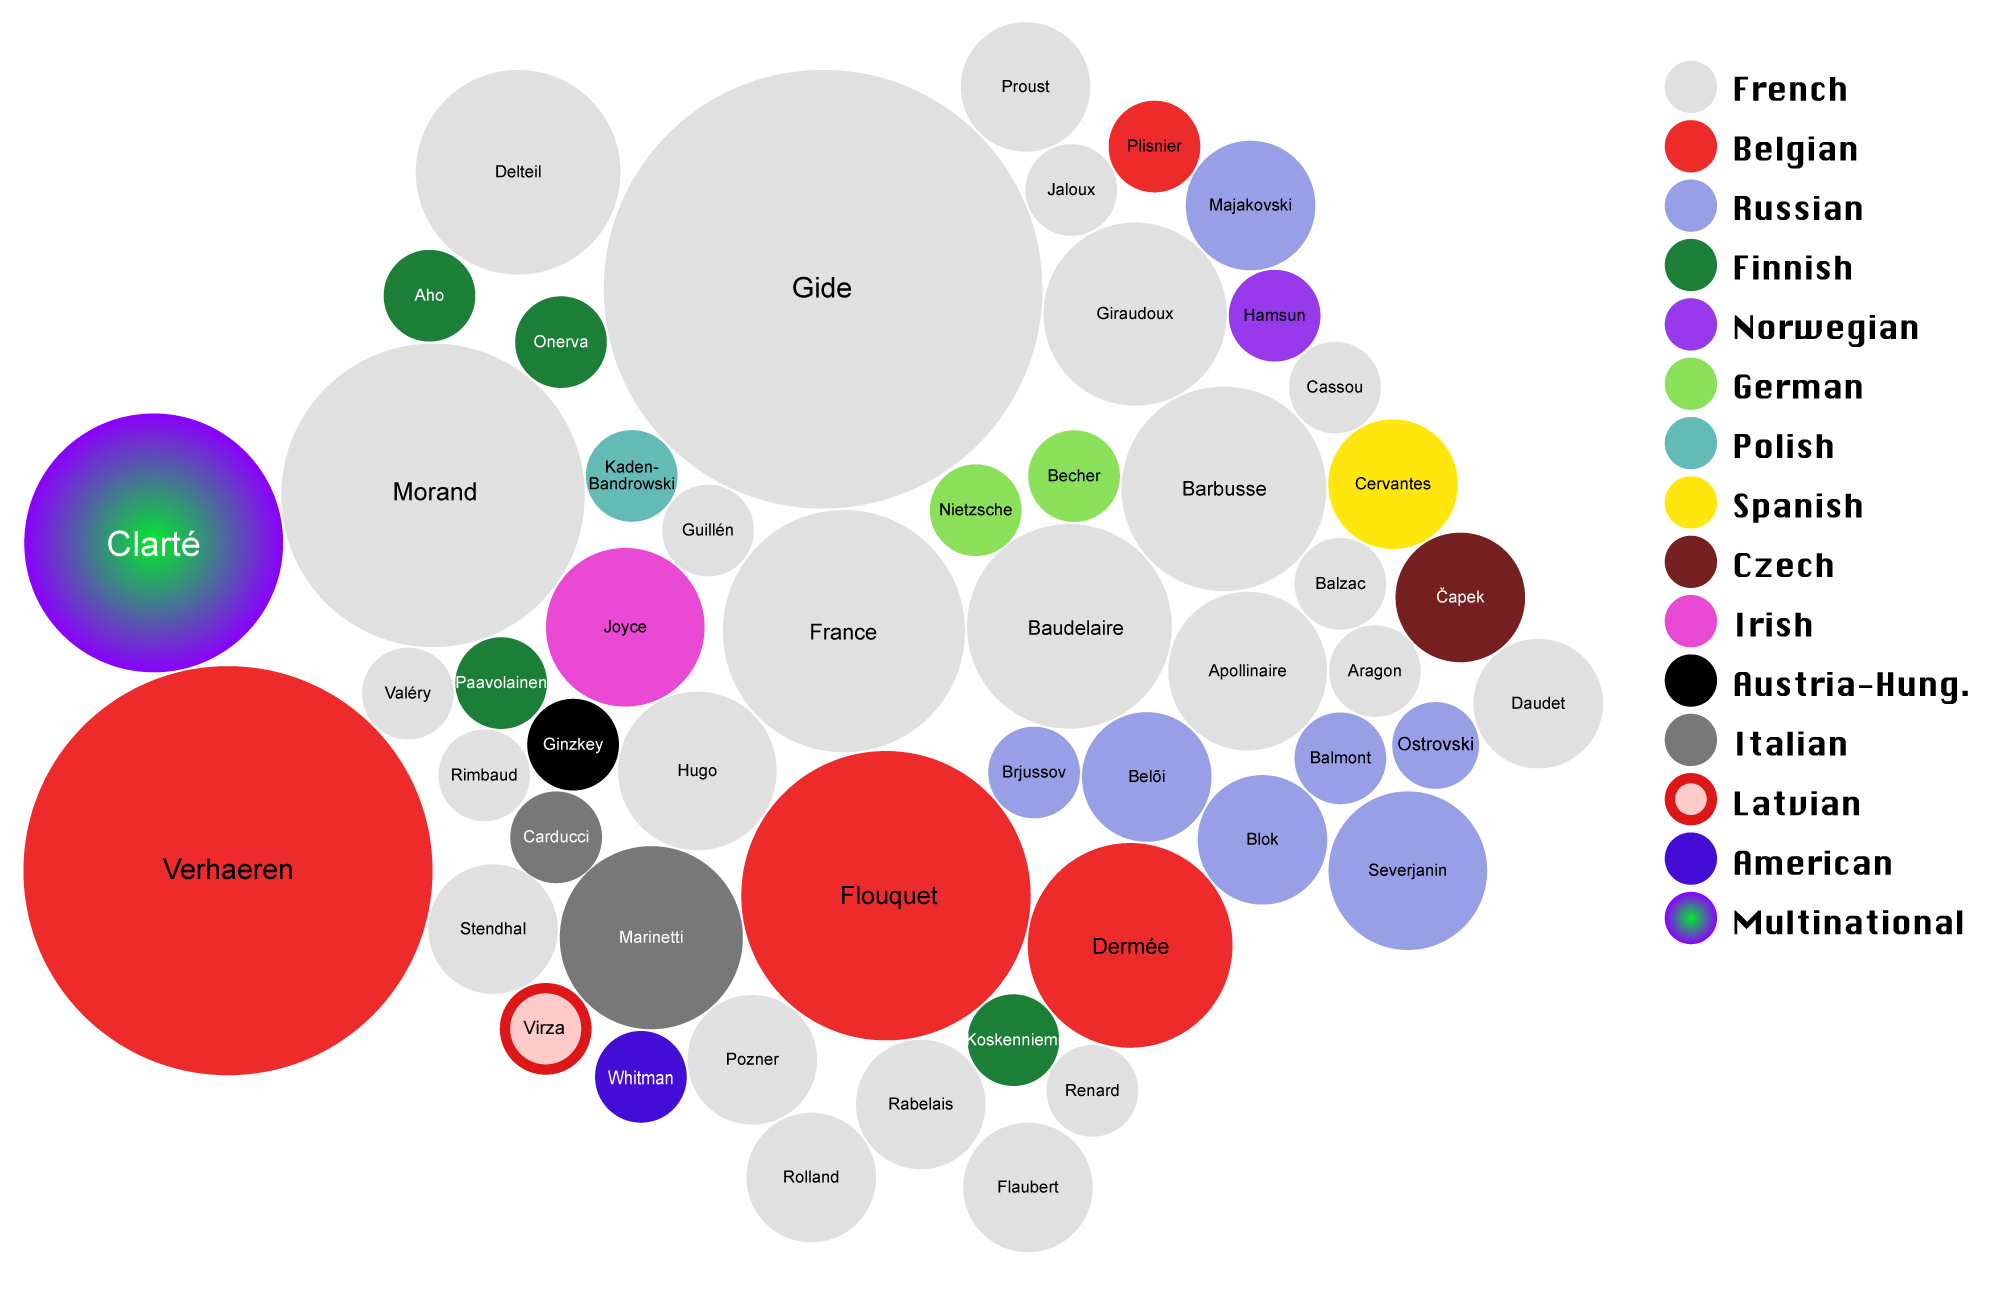
\includegraphics[width=\textwidth]{mummud}
  \caption{Foreign writers and countries mentioned in the correspondence based on the proper name index.  The size of the circle depends on the number of occurences in the corpus. The graph was generated using open source Javascript library from a predefined list of authors and number of letters to Barbarus. The colours were automatically assigned and later fine-tuned in visual editor.}
  \label{fig2}
\end{figure}


Query of KORP allows us to see the concordances of the Gide mentions, their absolute and relative frequency in the corpus, but not only. KORP allows us to organise the statistics by all the categories used in the corpus, including metadata categories. To know who of the authors and when mentioned Andre Gide, we only have to add those metadata categories (``sender'' and ``date'') to the statistics criteria; other metadata and linguistic categories can also be used for more sophisticated statistics that is connected to the concordances and broader context text blocks. 

\begin{table}
\caption{Statistics of mentioning Gide in KORP, organised by word form, sender and date.}\label{tab1}
\begin{tabular}{| l | l | l | r|}
  \hline
  word & sender & date & occurrences (absolute freq) \\
  \hline
  Gide'i & Semper & -- & 6.4 (2)\\
  Gide'i & Semper & 1926-12-13 & 3.2 (1)\\
  Gide'i & Semper & 1928-05-26 & 3.2 (1)\\
  Gide'il & Barbarus & 1928-05-26 & 3.2 (1)\\
  Gide'i & Semper & 1929-04-03 & 3.2 (1)\\
  Gide & Semper & 1929-05-06 & 3.2 (1)\\
  Gide'i-raamatule & Semper & 1929-04-03 & 3.2 (1)\\
  Gide'i & Semper & 1929-10-29 & 3.2 (1)\\
  Gide' & Semper & 1929-11-10 & 3.2 (1)\\
  Gide'i & Barbarus & 1929-12-08 & 3.2 (1)\\
  Gide & Semper & 1930-01-10 & 3.2 (1)\\
  Gide'i & Semper & 1930-10-13 & 3.2 (1)\\
  Gide'i & Barbarus & 1930-10-19 & 3.2 (1)\\
  Gide'i & Semper & 1931-07-03 & 3.2 (1)\\
  \hline
  &&Total:&51.5 (16)\\
\hline
\end{tabular}
\end{table}


From the statistics we see that it was mainly Semper who talked about Gide and the time interval is 1926 to 1930. It aligns well with the literary history: in 1928 Semper graduated as Master of Arts (magister artium) from the University of Tartu (with a master’s diploma in literary studies, ``The structure of the literary style of Andr\'e Gide'') and continued his work at the university as an aesthetics and stylistics lecturer.

\section{Current workflow}

At present stage we have applied the standard procedures for converting text into KORP-compatiblle corpus to the Correspondence corpus as well with some minor additions.  The standard procedure is a pipeline consisting of tokeniser, sentence splitter, morphological analyser (including POS-tagger and lemmatiser) and morphological disambiguator.  Sentence splitter was modified according to non-standard abbreviations found from the Correspondence texts, but morphological analyser was used with standard options: guesser and forced proper-name finder.

Sentence splitter and tokeniser are tools that determine the quality of the corpus.
They can be adjusted by properties of corpus and annotation aims, e.g. we can annotate a date as one token, or as a series of several tokens.  This would give different results of number of tokens and number of sentences.


Guesser makes the analyser find answers for words not in analyser's lexicon, and proper-name finder gives precedence to proper names, if analysis is ambiguous and word starts with a capital letter.  The corpus is not properly evaluated, but quick overview revealed at least two problems in POS tagging and lemmatisation.  First, the POS tagging seem to be too optimistic about proper names, and second, foreign words and phrases are analysed as Estonian.

We compared the number of proper names with manually disambiguated corpus, and found the general number to be rather normal.  Although being far more than in fiction, it fell between relative frequency of proper nouns in informational texts and journal texts (newspapers).  The over-estimation of proper nouns showed up at the introductory parts of the letters, where capitalised word ``Armas'' stands before name of the recipient.  The English equivalent would be ``Dear'' at the very beginning of letter.  Well, ``Armas'' is a first name used in Estonia, but it is a extremely rare one, and it was really never used as such in this correspondence.  We adjusted the workflow accordingly by switching off forced proper-name finder, and with some decline of the number of proper nouns, got rid of analysis of ``Armas'' as name.  How much did it affect the recall of proper names, needs some futher examination.

As it was mentioned before, both of the authors used foreign language in their letters as well.  Just now it is difficult to tell, how much, because the Estonian morphological analyser was too eager to find suitable analyses.  It would be possible to apply some language detecting tool before morphological analysis, but it is possible that foreign phrases are not so numerous and this strategy would generate too much noise.


\section{Future work and Perspectives}

The number of words and sentences in this corpus is rather big to tag it entirely manually, but at least by some extent it would be necessary.  Without manually annotated data it would be difficult, if not impossible, to evaluate automatic annotation that is trained on nowadays texts.  We are going to annotate at least some parts of the texts manually to find better methods to improve automatic analysis.


Such archival materials as a private correspondences of writers have a great cultural value, but promise an incredible linguistic importance as well. The elaborated search possibilities of KORP may be used to verify objectively, via linguistic analysis, the conclusions which have so far been drawn by using traditional methods of literary research, mainly using the well known method of slow close reading of the texts. 

Application of corpus linguistic methods in literary studies based on archival sources requires meticulous preparation of the material and transforming it into a text corpus. The text corpus of the correspondence of the writers, translators and friends Johannes Semper and Johannes Barbarus allows to go further with principally new type of research  questions, about the networks of the writers, or the ideas, that have influenced  the original works of both authors, leading more abstract semantic research. This could be the next phrase of the work with KORP.

% VÄLJA: Using the Semper \& Barbarus correspondence, we will study how such abstract semantic research problems can be clarified with the help of corpus linguistic methods and KORP. ETTEPANEK: 7. Current Workflow and future fork ja 8. For Conclusion 




%
% ---- Bibliography ----
%
% BibTeX users should specify bibliography style 'splncs04'.
% References will then be sorted and formatted in the correct style.
%
\bibliographystyle{splncs04}
\bibliography{laaketal}
%
\end{document}
